% arara: pdflatex: { shell: yes } until !found('log', '\\(?(R|r)e\\)?run (to get|LaTeX)')
\documentclass[a4paper,
DIV=13,
12pt,
BCOR=10mm,
department=FakEI,
%lucida,
%KeepRoman,
twoside,
parskip=half,
automark,
logostyle=flat,
%headsepline,
]{OTHRartcl}


\usepackage[ngerman,english]{babel}
\usepackage[hidelinks]{hyperref}

\date{\today}

\usepackage{cite}
\usepackage{amsmath,amssymb,amsfonts}
\usepackage{gensymb}
\usepackage{braket}






\usepackage[headsepline]{scrlayer-scrpage}
\pagestyle{scrheadings}
\automark[section]{section}
\automark*[subsection]{}

\documenttype{Project Report}

\title{Optimizing a source of polarization-entangled photons}
\author{Cosmin-Andrei Popan}
\studentid{3434442}
\department{Elektro- und Informationstechnik}
\studyprogramme{Bachelor Mechatronik}
\startingdate{16.03.2026}
\closingdate{27.07.2026}
\firstadvisor{Prof. Dr. Ioana Serban}
\secondadvisor{Prof. Dr. Robert Sattler}


% Hiermit trägt pdflatex die PDF-Metadaten des erzeugten Dokuments ein:
\hypersetup{pdftitle={\csname @title\endcsname{}},%
	pdfauthor={\csname @author\endcsname{}},%
	%pdfsubject={Optionaler Untertitel / englischer Titel},%
	%pdfkeywords={Optionale Schlüsselwörter}
	}

\begin{document}
\maketitle

\tableofcontents

\cleardoublepage


\section{Introduction}

This report documents the results of a research project carried out in the Quantum Technology Laboratory of the OTH Regensburg with the aim of optimizing an entangled photon source based on type I spontaneous parametric down-conversion (SPDC) in $\beta$-barium borate (BBO) crystals. Firstly, the theory of the SPDC process and the existing laboratory setup are described, highlighting the problems that need to be addressed. Afterwards, a new setup that aims to improve the photon coincidence rates is proposed and implemented, followed by a computer simulation written in Python that compares the measured photon rates with the ones predicted by the theory. Finally, an experiment to measure the Clauser-Horne-Shimony-Holt (CHSH) inequality is performed.

The results show a 25-fold improvement in the coincidence counts, with a CHSH statistic of $S = 2.36 \pm 0.04$, proving the presence of strong entanglement inside the photon pairs.




\section{Theoretical Background}

Spontaneous parametric down-conversion is a non-linear optical process that converts a photon of higher energy (called a pump photon) into a pair of photons of lower energy (called the signal and idler photons) subject to energy and momentum conservation. This constrant imposed by the conservation laws is referred to as phase-matching. The effect has first been observed in the 1960s and has since become a common technique for developing single-photon sources. One of the possible phase-matching schemes is Type-I SPDC, in which the signal and idler photons that are produced have the same polarization. The necessary conditions for this process can be met by using a birefringent crystal such as $\beta$-BBO \cite{spdc-intensity}.

\subsection{Birefringence in BBO crystals}

Birefringence is the optical property of some materials of having an index of refraction that depends on the polarization and direction of light. BBO is a birefringent crystal with a single optical axis. Light propagating through it with polarization perpendicular to its optical axis experiences the so-called ordinary index of refraction $n_o$ and is therefore known as an ordinary ray, whereas light whose polarization lies in the same plane as the optical axis experiences the direction-dependent extraordinary index of refraction $n_e(\theta)$, where $\theta$ is the angle between the extraordinary ray and the optical axis. A ray with a different polarization than the two cases described above gets split into an ordinary component and an extraordinary component, each experiencing the respective index of refraction. Denoting with $n_e = n_e(90 \degree)$ the refractive index experienced by the extraordinary ray that propagates perpendicular to the optical axis, the extraordinary refractive index for an arbitrary propagation direction is described by \cite{birefringence}:

\begin{equation}
    \frac{1}{n_e^2(\theta)} = \frac{\cos^2 (\theta)}{n_o^2} + \frac{\sin^2 (\theta)}{n_e^2}
    \label{n_e_theta}
\end{equation}


The ordinary and principal extraordinary refractive indices are described as functions of the wavelength by the Sellmeier equations \cite{sellmeier}:

\begin{equation}
    n_o^2 = 2.7359 + \frac{0.01878}{\lambda^2 - 0.01822} - 0.01354 \lambda^2
    \label{sellmeier_n_o}
\end{equation}

\begin{equation}
    n_e^2 = 2.3753 + \frac{0.01224}{\lambda^2 - 0.01667} - 0.01516 \lambda^2
    \label{sellmeier_n_e}
\end{equation}


\subsection{Spontaneous phase-matching in BBO crystals}

Type-I spontaneous parametric down-conversion is the process whereby a pump photon of frequency $\omega_p$ enters the BBO crystal as an extraordinary ray at an angle $\theta_m$ (called the phase-matching angle) with respect to the optical axis and gets converted into a pair of signal-idler photons with frequencies $\omega_s$, $\omega_i$ that exit the crystal as ordinary rays. Therefore, the polarization of the signal and idler rays is perpendicular to that of the pump. Figure \ref{fig:spdc_feynman} depicts the corresponding Feynman diagram. Using $E=\hbar \omega$ and $\mathbf{p} = \hbar \mathbf{k}$, the energy and momentum conservation can be expressed as:

\begin{equation}
    \omega_p = \omega_s + \omega_i
    \label{energy_conservation}
\end{equation}

\begin{equation}
    \mathbf{k}_p = \mathbf{k}_s + \mathbf{k}_i
    \label{momentum_conservation}
\end{equation}

where $\mathbf{k}$ are the respective wave vectors, with the dispersion relation $k=\frac{n\omega}{c}$ \cite{spdc-intensity}.

\begin{figure}[htbp]
\centerline{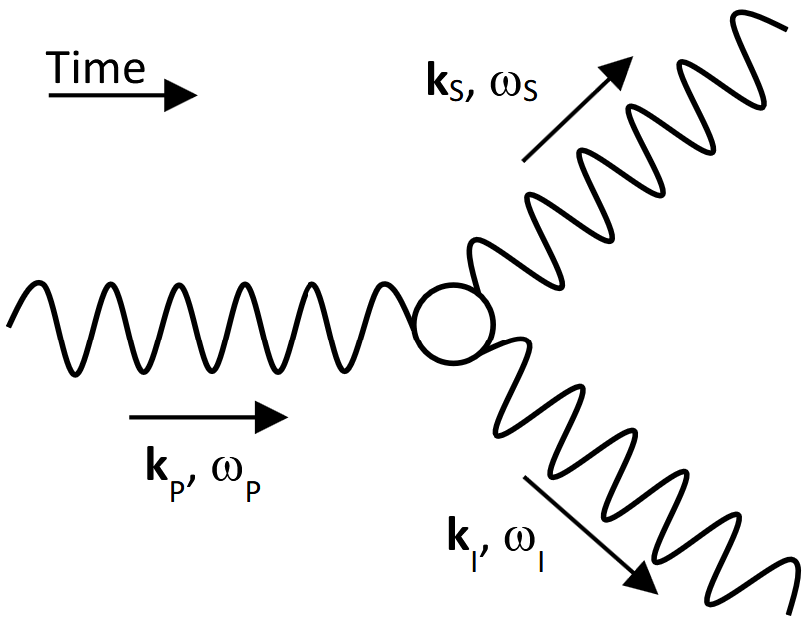
\includegraphics[scale=0.5]{spdc_feynman.png}}
\caption{Feynman diagram for SPDC pair production. Figure taken from \cite{spdc_feynman}.}
\label{fig:spdc_feynman}
\end{figure}

Let $\theta_s'$ and $\theta_i'$ be the angles formed by the pump ray with the signal and idler rays, respectively (inside the crystal). In the case of degenerate down-conversion, $\omega_s = \omega_i = \frac{\omega_p}{2}$. The momentum conservation in the transverse direction gives $\frac{n_o \omega_s}{c} \cdot \sin (\theta_s') = \frac{n_o \omega_i}{c} \cdot \sin (\theta_i')$, which means $\theta_s' = \theta_i'$. With $\lambda_s = 2 \lambda_p$, longitudinal momentum conservation becomes:

\begin{equation}
    n_e(\lambda_p, \theta_m) = n_o(2\lambda_p) \cdot \cos (\theta_s')
    \label{momentum_conservation_degenerate}
\end{equation}


Figure \ref{fig:spdc_cone} shows the typical configuration for type I phase matching. A BBO crystal is cut thinly in such a way, that its optical axis makes the angle $\theta_m$ with the normal to its surface. Thus, a pump beam that hits the crystal under normal incidence will produce degenerate photon pairs symmetrically under the angle $\theta_s'$ given by \eqref{momentum_conservation_degenerate}. The signal and idler rays are then refracted at the air-crystal boundary and leave the crystal under the laboratory angle $\theta_sL$ with the pump beam direction:

\begin{equation}
    n_o(2\lambda_p) \cdot \sin (\theta_s') = \sin (\theta_s)
    \label{refraction_signal}
\end{equation}

Due to rotational symmetry about the pump beam direction, the photons emerge from the crystal on a cone with half-opening angle $\theta_s$, where photons from the same pair are situated diametrically opposite from each other.


\begin{figure}[htbp]
\centerline{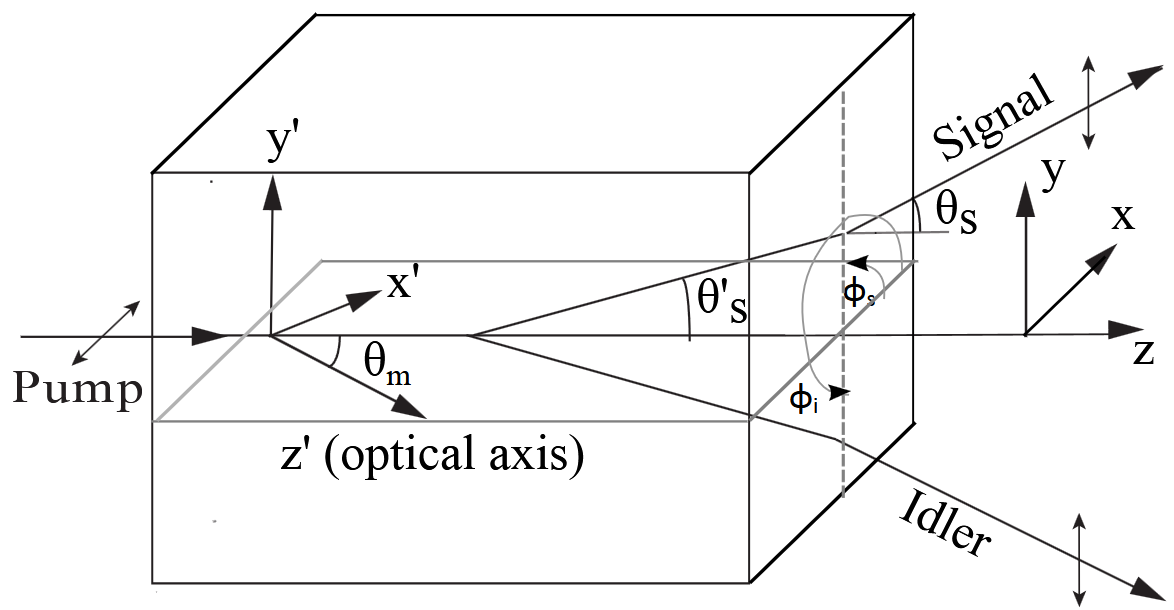
\includegraphics[scale=0.75]{spdc_cone.png}}
\caption{Spatial distribution of the down-conversion emission for type I phase-matching. Figure taken from \cite{spdc-intensity}.}
\label{fig:spdc_cone}
\end{figure}


As such, capturing the photons is only a matter of placing the detectors at the correct positions predicted by equations \eqref{momentum_conservation_degenerate} and \eqref{refraction_signal}. However, these calculations do not contain any information about the expected number of down-converted photons that will be generated, nor do they take into account the effects of imperfect phase-matching.




\subsection{Computing SPDC intensity}

A method for computing the intensity of spontaneous parametric down-conversion, taking into account all of the emission wavelengths and directions is presented in \cite{spdc-intensity}. This paper takes into account imperfect phase-matching by considering the mismatch wave vector $\mathbf{\Delta k} = \mathbf{k}'_s + \mathbf{k}'_i - \mathbf{k}'_p$, which gets decomposed into longitudinal ($\Delta k_z$) and transverse ($\kappa$) components:

\begin{equation}
    \Delta k_z = \sqrt{{k'_s}^2 - \kappa_s^2} + \sqrt{{k'_i}^2 - \kappa_i^2} - k'_p
    \label{mismatch_vector_longitudinal}
\end{equation}

\begin{equation}
    \kappa = \kappa_s + \kappa_i
    \label{mismatch_vector_transverse}
\end{equation}

Here $k'_s = \frac{n_s \omega_s}{c}$, $k'_i = \frac{n_i \omega_i}{c}$, $k'_p = \frac{n_p \omega_p}{c}$ are the wavenumbers inside the crystal for the signal, idler and pump waves, respectively.

The rate of down-converted photons of vacuum wavelength $\lambda_s$ emitted under the laboratory angle $\theta_s$ is given by\footnote{In equation (9) of \cite{spdc-intensity}, the azimuthal angle differential $d\phi$ is omitted, however the expression does get integrated over the azimuthal angle during the numerical integration step. Here it has been included in the equation for consistency.}:

\begin{equation}
    N_s(\lambda_s, \theta_s) = \frac{2\pi \sqrt{2\pi}\, \hbar\, d_{eff}^{\,2}\, \omega_p\, L^2\, N_p}{\epsilon_0\, n_s\, n_i\, n_p\, \lambda_s^5\, \lambda_i}\, \sin(2\theta_s)\, d\lambda_s\, d\theta_s\, d\phi \int d\xi_i\, e^{-\frac{1}{2}(\xi_s - \xi_i)^2} \cdot \operatorname{sinc}^2\!\left(\frac{1}{2}\, L\, \Delta k_z\right)
    \label{spdc_intensity}
\end{equation}

where $d_{eff}$ is the effective second-order nonlinear coefficient of the crystal, L the crystal length, $N_p = \frac{P_p}{\hbar \omega_p}$ the pump flux, $n_s, n_i, n_p$ the respective refraction indices, and $d \lambda_s, d\theta_s, d\phi$ are the infinitesimal variations in wavelength, signal angle and azimuthal angle over which the photon flux is calculated. Furthermore, $\xi_i = \kappa_i W$ and $\xi_s = \kappa_s W$ are the dimensionless transverse momenta associated with the signal and idler waves, with $W$ being the pump beam radius.

This expression will be used in a later section to compute the theoretically expected count rates and compare them to the measured rates. 


\subsection{Generating polarization-entangled photons}

Spontaneous parametric down-conversion can be used to obtain pairs of polarization-entangled photons by replacing the single BBO crystal with a pair of BBO crystals with optical axes perpendicular to each other, as shown in Figure \ref{fig:crystal_sandwich_cones}. Positioning the axis of the first crystal horizontally and that of the second crystal vertically and polarizing the pump laser to $45\degree$ allows for an equal probability of each pump photon being down-converted in either of the two crystals. A signal-idler pair generated in the first crystal will then be vertically polarizer, and a pair generated in the first crystal will be horizontally polarized.

If the setup is aligned in such a way, that the photons emitted by either crystal are captured by the same detectors, one cannot distinguish where a detected photon came from, hence the polarization of a given photon is in a superposition. Since photons in a pair must have the same polarization, they are in the entangled Bell state \cite{ultrabright_source_entangled}:

\begin{equation}
    \ket{\Phi^+} = \frac{1}{\sqrt{2}} \bigl(\ket{HH} + \ket{VV}\bigr)
    \label{bell_state}
\end{equation}

where $\ket{H}$ denotes horizontal and $\ket{V}$ denotes vertical polarization (assuming no phase difference between photons emitted by different crystals).

\begin{figure}[htbp]
\centerline{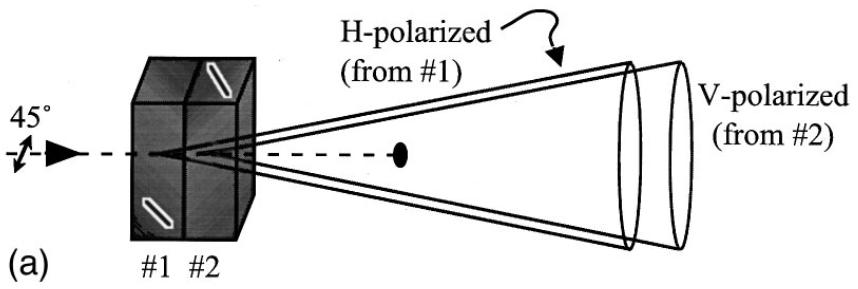
\includegraphics[scale=0.75]{crystal_sandwich_cones.png}}
\caption{Method to produce polarization-entangled photons
from two identical down-conversion crystals, oriented at 90° with
respect to each other. Figure taken from \cite{ultrabright_source_entangled}.}
\label{fig:crystal_sandwich_cones}
\end{figure}


\subsection{The Clauser-Horne-Shimony-Holt (CHSH) inequality}

CHSH is a version of Bell's inequality that can be used to test the entanglement of particles. This inequality holds only in local realistic theories, while quantum mechanics predicts it can be violated. By experimentally measuring a violation, one can prove that the state being measured is entangled, a quantum mechanical property that cannot by explained by classical physics.

To apply this to the setup described above, rotatable linear polarizers can be placed such that the down-converted photons are forced to pass through them before arriving at the detectors. The single-photon detectors are then connected to a coincidence counter, that counts the number of simultaneous detections within a small time window. Using two angle settings for each of the polarizers ($\alpha, \alpha'$ for the first one, $\beta, \beta'$ for the second one), the CHSH inequality is \cite{qued_manual}:

\begin{equation}
    |S(\alpha, \alpha', \beta, \beta')| = \left| E(\alpha, \beta) + E(\alpha', \beta) - E(\alpha, \beta') + E(\alpha', \beta') \right| \leq 2
    \label{CHSH}
\end{equation}

Here $E(\alpha, \beta)$ denotes the normalized expectation value of correlations between the measurements. Denoting with $C(\alpha, \beta)$ the coincidence count obtained with the polarizers set to angles $\alpha$ and $\beta$, respectively, this can be computed as \cite{qued_manual}:

\begin{equation}
    E(\alpha, \beta) = \frac{C(\alpha, \beta) - C(\alpha, \beta_\perp) - C(\alpha_\perp, \beta) + C(\alpha_\perp, \beta_\perp)}{C(\alpha, \beta) + C(\alpha, \beta_\perp) + C(\alpha_\perp, \beta) + C(\alpha_\perp, \beta_\perp)}
    \label{CHSH_correlation}
\end{equation}

where $\alpha_\perp = \alpha + 90\degree$ and $\beta_\perp = \beta + 90\degree$.

Furthermore, the standard deviation of $S$ can be computed using:

\begin{equation}
    \Delta S(\alpha, \alpha', \beta, \beta') = \sqrt{\sum_{a=\alpha,\alpha'} \sum_{b=\beta,\beta'} \Delta E(a,b)^2}
    \label{CHSH_std_deviation}
\end{equation}

\begin{multline}
    \Delta E(a,b) = 2 \frac{\left[ C(a,b) + C(a_\perp, b_\perp) \right] \left[ C(a, b_\perp) + C(a_\perp, b) \right]}{\left( C(a,b) + C(a, b_\perp) + C(a_\perp, b) + C(a_\perp, b_\perp) \right)^2} \\
    \times \sqrt{\frac{1}{C(a,b) + C(a_\perp, b_\perp)} + \frac{1}{C(a, b_\perp) + C(a_\perp, b)}}
    \label{CHSH_correlation_std_deviation}
\end{multline}


\subsection{Accidental coincidences}

As highlighted above, the CHSH experiment relies on measuring the coincidence counts with different polarization settings. This is, in fact, necessary for any experiment performed using the down-converted photon pairs, because the only way to tell that a photon pair was produced is to detect both  photons at the same time. It is important to note that the coincidence rate will be different than the individual rates of the detectors in a real experiment, because the detectors have dark counts and because there will always be a certain amount of stray light entering them. The coincidence count much less affected by these random events because it is much more unlikely for two such events to occur at almost the same time, triggering both detectors at once.

For a coincidence time window $\Delta t_w$, an integration time of 1 s, and individual counts $N_1$ and $N_2$ assumed to be random and independent, the rate of accidental coincidences is:

\begin{equation}
    N_{12,acc} = N_1 N_2\, \Delta t_w
    \label{accidental_coincidences}
\end{equation}











\section{Existing setup and possible issues}

\subsection{Existing setup}

At the beginning of this project, a source of entangled photons based on Type I SPDC had already been built at the Quantum Technology Laboratory of the OTH Regensburg. A schematic drawing of the existing setup is presented in Figure \ref{fig:old_setup}.

The setup was mounted on an optical table and included two different pump lasers that could be used individually, a 10 mW one that was not temperature stabilized and a 20 mW temperature stabilized one (diode Thorlabs L405P20, mount Thorlabs LDM9T), both operating at 405 nm. The pump beam was directed onto a pair of 0.1 mm thick BBO crystals (Newlight Photonics PABBO5010-405(I)-HA3) and then into a beamtrap. The down-converted photons exiting the crystals were reflected by two mirrors (Thorlabs PF10-03-P01, PF20-03-P01), passed through colored glass filters (Thorlabs FGL610) and were picked up by optical fibers (Thorlabs MR17L01) with the help of a lens mounted in the fiber couplers. These were connected to a detector box with builtin avalanche photodiode (APD) detectors and coincidence counter (qutools quED).


\begin{figure}[htbp]
\centerline{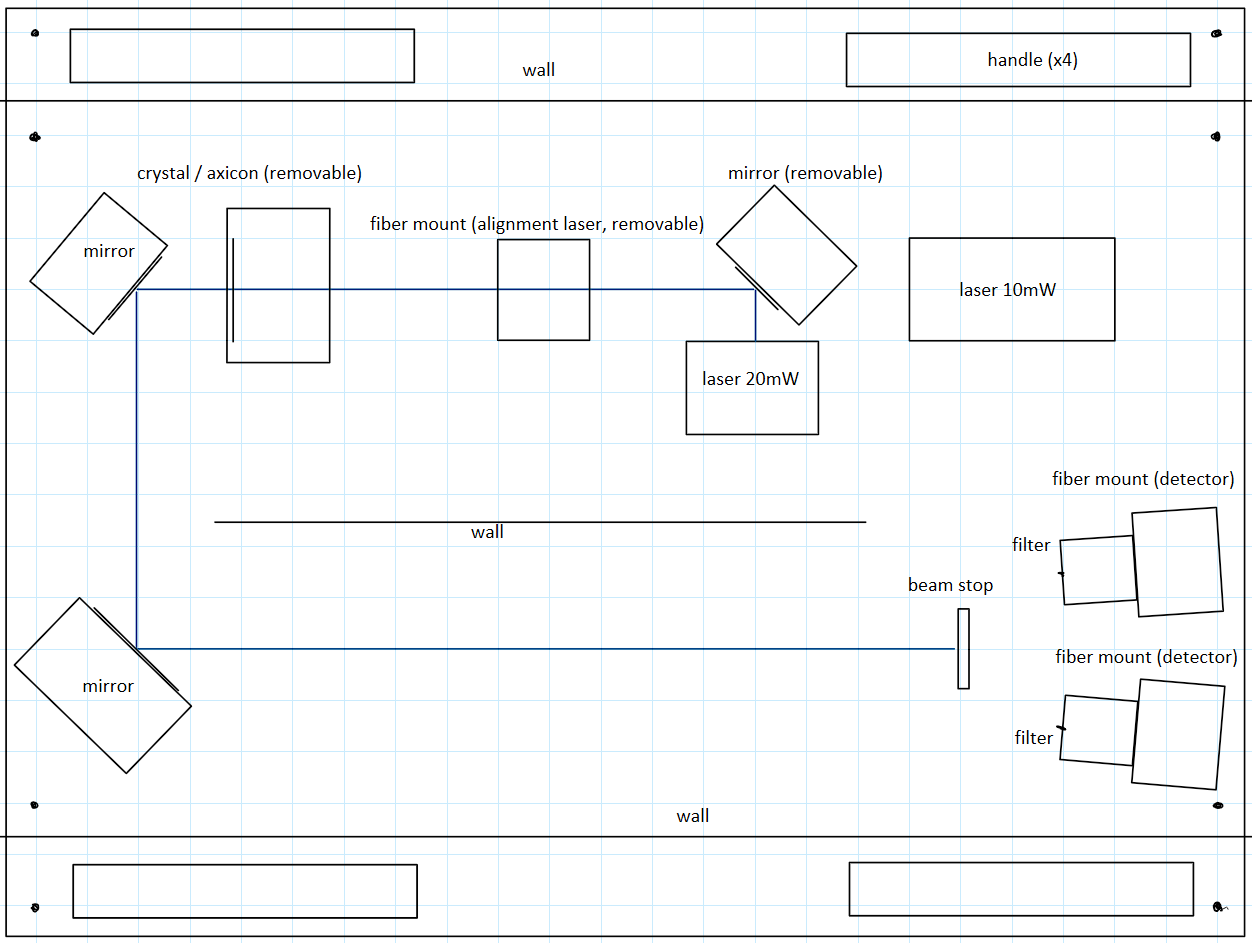
\includegraphics[scale=0.7]{old_setup.png}}
\caption{Existing setup (to scale)}
\label{fig:old_setup}
\end{figure}

The alignment of the setup was performed by using a separated red alignment laser, which could be temporarily mounted onto the same beampath using a fiber coupler. The crystal could then be replaced by an axicon (Thorlabs AX123), which is a special optical component that turns a beam of light that hits it in the center under normal incidence into a cone of light, with a half opening angle of 3$\degree$. This perfectly matches the cone that is generated by SPDC and can be used to visually position the detectors and filters.

The mirrors, fiber mounts, crystal and axicon are all mounted using kinematic mounts that allow precise rotation about the vertical and horizontal axes.

The following measurements were obtained using this setup (20 ns time window, 1 s integration time):
\begin{itemize}
    \item single count rate, detector 1: $\sim\! 71000$ counts/s
    \item single count rate, detector 2: $\sim\! 22000$ counts/s
    \item coincidence count rate: $\sim\! 45$ counts/s
\end{itemize}

It can be observed that the coincidence rate is much lower than the individual rates. Applying equation \eqref{accidental_coincidences} with $\Delta t_w = 20$ ns results in 31 expected accidental coincidences per second. This means that at most a small percentage of the measured coincidences are truly the result of spontaneous parametric down-conversion.

Furthermore, a measurement of the CHSH inequality had previously been performed, with inconclusive results. The goal of this project is to find possible issues with the setup, improve the coincidence rate, and confirm a proper entangled state using CHSH.


\subsection{Issues to be addressed}

\subsubsection{Filters}

Noticing the low proportion of coincidence counts to single counts, a first idea is to block out more of the stray light that might be entering the fibers and causing random detections. Indeed, removing the crystal pair completely from the setup and replacing it with a polarizer, which serves the single purpose of scattering a small portion of the pump beam in random directions, results in very similar rates to the ones obtained with the crystals in place. This confirms that the vast majority of the detected photons are scattered pump photons that are not being sufficiently blocked by the filters.

A simple solution is replacing the colored glass filters with 810 nm bandpass filters, with a full width at half maximum (FWHM) of 10 nm (Thorlabs FBH810-10), which were already available in the lab. Measuring again shows a vastly different picture: 1400/800 single counts with 0 coincidences (with the crystals mounted). Taking into account the detector dark counts, this confirms that the bandpass filters are much better at removing the unwanted stray radiation. It also shows that the setup currently produces no actual down-converted photons.

An important observation is that the bandpass filters have been used previously, but the measurements with them have always resulted in less than 5 coincidences per second, even after multiple attempts at alignment. This suggests that there is a deeper underlying problem that makes proper alignment impossible with the current setup.


\subsubsection{Pump laser wavelength deviations}

A possible problem ??


dark couunts, cover setup with cloth, mention 810 nm at the beninging







\cleardoublepage
\appendix
\listoffigures

%\cleardoublepage

\bibliographystyle{plain}
\bibliography{refs}

%\cleardoublepage
\makedeclaration

\end{document}
